\documentclass{article}

\usepackage{../repsty}

\begin{document}
\title{Polarization analysis}
\author{Alexander Aksentev}
\maketitle
	
\section{Life-time analysis}
Life-time analysis was done on the basis of the data from run 7079. The data were fitted from 30 to 250 seconds of run time. In Figure~\ref{fig:ROOT-AllRings} are shown (left to right): the polarization and cross-section fits (constant) for each ring separately, and the cross-section from all rings as a function of time.
\begin{figure}[h]
	\centering
	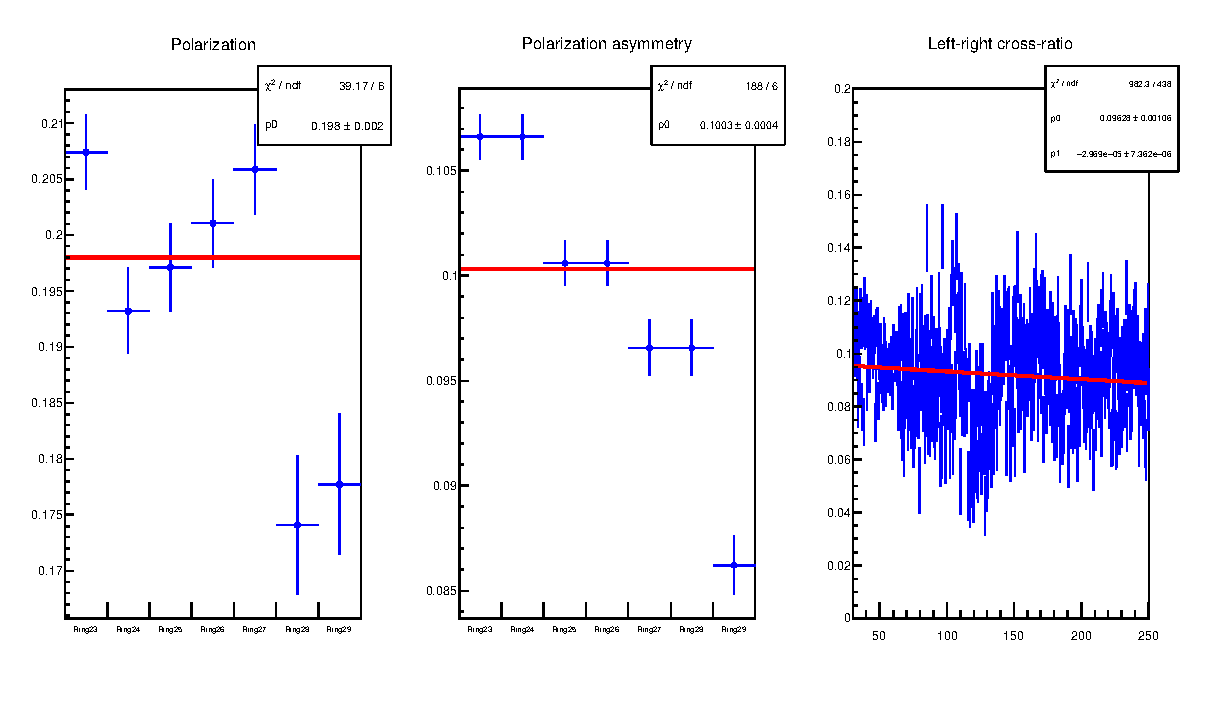
\includegraphics[scale=.35]{PolAna-ROOT-all}
	\caption{Polarization and  cross section data.\label{fig:ROOT-AllRings}}
\end{figure}

We fitted the linear model to the cross-ratio data. Polarization life-time is then estimated as $\hat{\tau} = -1/\hat{\beta}$, where $\hat{\beta}$ is the slope estimate of the fit. This was done for each ring separately. The results are in Figure~\ref{fig:R-SepRings}. Rings 10 and 15 (24 and 29 respectively) were excluded for due to high uncertainty in their estimates. The fit results are summarized in Table~\ref{tbl:FitRes}.

\begin{figure}[h]
	\centering
	\includegraphics[scale=.8]{PolAna-CRLTvsCR0}
	\caption{Cross-ratio life-time vs initial value (upper panel), and the density distribution of the life-times (lower panel).\label{fig:R-SepRings}}
\end{figure}

\begin{table}[h]
	\centering
	\caption{Fit results.\label{tbl:FitRes}}
	\begin{tabular}{rrrrrrrr}
		\hline
		Ring &    $CR_0$ & $\sigma(CR_0)$ & $\hat{\tau}_{CR} (sec)$ & $\sigma(\hat{\tau}_{CR})(sec)$ & $\hat{P}_0$ & $\sigma(\hat{P}_0)$ & $\chi^2_\nu$\\ \hline
		   9 & 0.1082970 &     0.00219011 &                74643.02 &                      85463.586 &    0.256513 &          0.00257090 & 1.0091941\\
		  10 & 0.1023290 &     0.00222041 &                72182.36 &                      80885.635 &    0.262250 &          0.00262840 & 0.9457489\\
		  11 & 0.1087920 &     0.00295643 &                11083.84 &                       2393.469 &    0.252412 &          0.00271611 & 1.3768082\\
		  12 & 0.0923701 &     0.00288661 &                20322.97 &                       8346.538 &    0.257666 &          0.00277264 & 1.0893151\\
		  13 & 0.0810401 &     0.00323987 &                50478.54 &                      57822.875 &    0.253199 &          0.00347838 & 1.1641644\\
		  14 & 0.0839395 &     0.00318726 &                22975.30 &                      11790.275 &    0.260313 &          0.00357611 & 1.1479155\\
		  15 & 0.0618035 &     0.00491475 &               -45611.91 &                      71725.457 &    0.237312 &          0.00384081 & 1.1738242\\ \hline
	\end{tabular}
\end{table}

The three more precise estimates (rings 11, 12, and 14) lead to the conservative estimate of $\tau_{CR}\approx 11$ thousand seconds.

\end{document}